Para cada uno de los circuitos que se muestran en las figuras \ref{fig:filtro-variables-de-estado}, \ref{fig:filtro-sallen-key} y \ref{fig:filtro-realimentacion-multiple}, se debe realizar el siguiente proceso de preparación:

\begin{enumerate}
    \item Obtener su modelo circuital de entrada a cada una de sus salidas, observar la importancia de la función de transferencia.
    \item Especificar los componentes necesarios, en cada filtro, para obtener frecuencias de corte de $2.7 kHz$ con factor de amortiguamiento de 0.707, con ganancia de 2 en la salida pasa bajos.
    \item Verificar sus diseños, mediante simulación, comparando la respuesta en frecuencia obtenida, con el diagrama asintótico de Bode de cada filtro. Determine la ganancia de cada filtro a las frecuencias en las que planea medir la respuesta en frecuencia.
    \item Por simulación obtener las formas en cada salida al inyectar señales cuadradas con frecuencia tal, que su tercera armónica, coincida con la frecuencia de corte indicadas. Explicar a que se deben las formas de onda obtenidas.
    \item Elabore la hoja de datos necesaria para recabar las mediciones y los datos del montaje, en los ensayos descritos por usted previamente.
\end{enumerate}

\begin{figure}[ht]
    \centering
    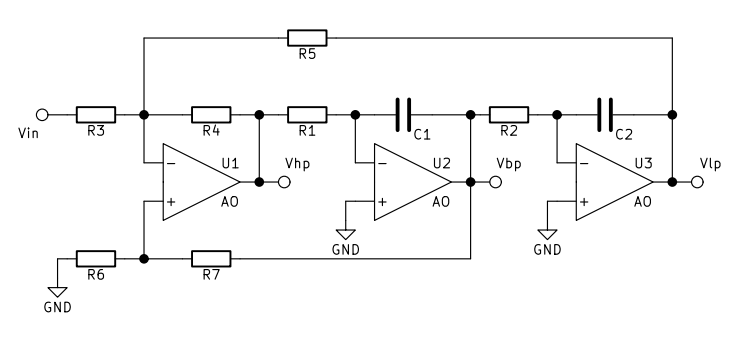
\includegraphics[width=0.8\textwidth]{filtro-variables-de-estado.png}
    \caption{Filtro de variables de estado}
    \label{fig:filtro-variables-de-estado}
\end{figure}

\begin{figure}[ht]
    \centering
    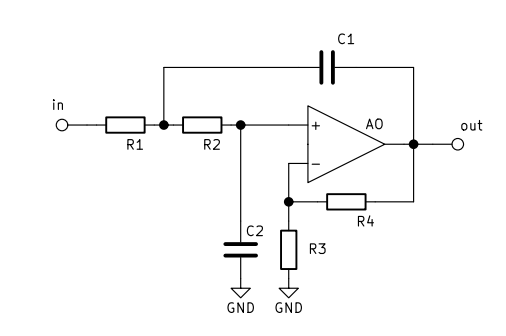
\includegraphics[width=0.6\textwidth]{filtro-sallen-key.png}
    \caption{Filtro pasa bajos con topología de Sallen-Key}
    \label{fig:filtro-sallen-key}
\end{figure}

\begin{figure}[ht]
    \centering
    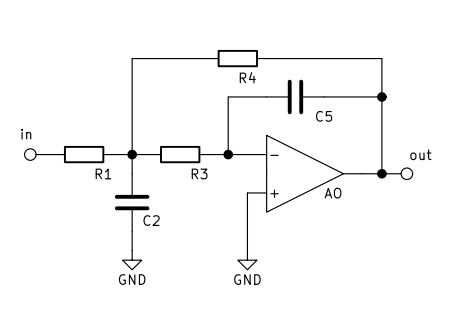
\includegraphics[width=0.5\textwidth]{filtro-realimentacion-multiple.png}
    \caption{Filtro pasa bajos con realimentación múltiple}
    \label{fig:filtro-realimentacion-multiple}
\end{figure}

\FloatBarrier
\subsubsection{Filtro de variables de estado}

De la figura \ref{fig:filtro-variables-de-estado} se observa que las etapas con los amplificadores $U2A0$ y $U3A0$ corresponden a a integradores con ganancia $A = \frac{1}{RCs}$, por lo tanto podemos expresar $V_{bp}$ y $V_{lp}$ como:

\begin{equation}
    \VLP = \frac{1}{R_2 C_2 s}V_{bp}
    \label{eq:vo-integrador-2}
\end{equation}

\begin{equation}
    \VBP = \frac{1}{R_1 C_1 s}V_{hp}
    \label{eq:vo-integrador-1}
\end{equation}

El amplificador $U1A0$ recibe las señales $V_{in}$, $V_{BP}$ y $V_{R6}$, teniendo en cuenta que la caída de tensión en $R_6$ es:

$$V_{R6} = \frac{R_6}{R_6 + R_7}\VBP$$

podemos expresar la tensión $\VHP$ cómo:

\begin{equation}
    \VHP = -\frac{R_4}{R_3}\VIN -\frac{R_4}{R_5}\VLP + \left (1 + \frac{R_4}{R_3 \parallel R_5}\right )\frac{R_6}{R_6 + R_7}\VBP
    \label{eq:vhp-uno}
\end{equation}

Ahora, usando las ecuaciones \ref{eq:vo-integrador-1} y \ref{eq:vo-integrador-2} podemos expresar la tensión de salida $\VBP$ cómo:

\begin{equation}
    \VLP = \frac{1}{R_2 C_2 s} \frac{1}{R_1 C_1 s}\VHP
    \label{eq:vlp-ambos-integradores}
\end{equation}

Sustituyendo la ecuación \ref{eq:vo-integrador-1} en la ecuación \ref{eq:vhp-uno} obtenemos:

\begin{equation}
    \VHP = -\frac{R_4}{R_3}\VIN -\frac{R_4}{R_5}\VLP + \WrapParenthesis{1 + \frac{R_4}{R_3 \parallel R_5}}\frac{1}{R_1 C_1 s}\frac{1}{R_2 C_2 s}\frac{R_6}{R_6 + R_7}\VHP
    \label{eq:vhp-dos}
\end{equation}

Despejando $\VHP$:

\newcommand{\VHPEq}{
    - \frac{\frac{R_4}{R_3}\VIN + \frac{R_4}{R_5}\VLP}{1 + \frac{R_6}{R_6 + R_7} \WrapParenthesis{1 + \frac{R_4}{R_3 \parallel R_5}}\frac{1}{R_1 C_1 s}}
}
\newcommand{\Numerador}{\frac{R_4}{R_3}\VIN + \frac{R_4}{R_5}\VLP}

\newcommand{\Denominador}{1 + \frac{R_6}{R_6 + R_7} \WrapParenthesis{1 + \frac{R_4}{R_3 \parallel R_5}}\frac{1}{R_1 C_1 s}}



\begin{equation}
    \VHP = \VHPEq
    \label{eq:vhp-tres}
\end{equation}

De la ecuación \ref{eq:vhp-tres} podemos definir el denominador como $D_1$:

\begin{equation}
    D_1 = \Denominador
    \label{eq:d1}
\end{equation}



Sustituyendo la ecuación \ref{eq:vhp-tres} en la ecuación \ref{eq:vlp-ambos-integradores} obtenemos:

\begin{equation}
    \VLP = - \frac{1}{R_2 C_2 s} \frac{1}{R_1 C_1 s}\WrapParenthesis{\frac{\Numerador}{D_1}}
    \label{eq:vlp-ambos-integradores-sustituido}
\end{equation}

Despejando $\VLP / \VIN$, tenemos:

\begin{equation}
    \frac{\VLP}{\VIN} = - \frac{\cancel{\frac{1}{R_2 C_2 s}} \cancel{\frac{1}{R_1 C_1 s}} \frac{R_4}{R_3}}{\WrapParenthesis{D_1 R_2 C_2 R_1 C_1 s^2 + \frac{R_4}{R_5}}\cancel{\frac{1}{R_2 C_2 s}} \cancel{\frac{1}{R_1 C_1 s}}}
\end{equation}

Cancelando $\frac{1}{D_1}$:

\begin{equation}
    \frac{\VLP}{\VIN} = - \frac{R_4}{R_3}\frac{1}{\WrapParenthesis{D_1 R_2 C_2 R_1 C_1 s^2 + \frac{R_4}{R_5}}}
    \label{eq:vlp-vin-uno}
\end{equation}

Ahora, sustituyendo $D_1$ (ecuación \ref{eq:d1}) en \ref{eq:vlp-vin-uno} obtenemos:

\begin{equation}
    \frac{\VLP}{\VIN} = - \frac{R_4}{R_3}\frac{1}{\WrapParenthesis{\WrapBrackets{\Denominador} R_2 C_2 R_1 C_1 s^2 + \frac{R_4}{R_5}}}
    \label{eq:vlp-vin-dos}
\end{equation}

Por simplificación podemos decir que:

\begin{align*}
    R_1 = R_2 \\
    C_1 = C_2
\end{align*}

Por lo tanto, podemos reescribir la ecuación \ref{eq:vlp-vin-dos} como:


\begin{equation}
    \frac{\VLP}{\VIN} = - \frac{R_4}{R_3 R_1^2 C_1^2} \frac{1}{s^2 + s \frac{R_6}{R_6 + R_7} \frac{R_3 \parallel R_5 + R_4}{R_3 \parallel R_5} \frac{1}{C_1 R_1} + \frac{R_4}{R_5 R_1^2 C_1^2}}
\end{equation}

Usando la formula de filtros pasa bajos, tenemos:

\begin{align}
    \freqCorte^2 &= \frac{R_4}{R_5 R_1^2 C_1^2} \label{eq:freq-corte-variable-de-estado} \\
    \howoSQT &= - \frac{R_4}{R_3 R_1^2 C_1^2} \label{eq:howo-sqt-variable-de-estado} \\
    \gananciaFiltro &= -\frac{R_5}{R_3} \label{eq:ganancia-filtro-variable-de-estado}
\end{align}

\begin{equation}
    2\factorAmortiguamiento\freqCorte = \frac{R_6}{R_6 + R_7} \frac{R_3 \parallel R_5 + R_4}{R_3 \parallel R_5} \frac{1}{C_1 R_1} 
    \label{eq:factor-amortiguamiento-variable-de-estado}
\end{equation}

Sustituyendo los valores deseados tenemos:
\begin{align*}
    \gananciaFiltro &= -2 = -\frac{R_5}{R_3} \\
    R_5 &= 2 R_3 \\
\end{align*}

por lo tanto:

$$ R_3 \parallel R_5 = R_3 \parallel 2 R_3 = \frac{2}{3}R_3 $$

ahora, en primer lugar escogeremos un valor para $C_1$ ya que es el componente que menor opciones tiene:

\begin{equation*}
    \boxed{C_1 = 10 nF}
\end{equation*}

por simplificación diremos que $R_5 = R_4$, por tanto:

\begin{equation}
    \freqCorte = \frac{1}{R_1 C_1}
\end{equation}

de este modo, partiendo de la ecuación \ref{eq:freq-corte-variable-de-estado} obtenemos:

\begin{align*}
    R_1 &= \frac{1}{\freqCorte C_1} \\
    R_1 &= \frac{1}{2\pi 2.7\times 10^3 \cdot 10\times 10^{-9}} \\
\end{align*}
\begin{equation}
    \boxed{R_1 = R_2 = 5894 \Omega}
\end{equation}

Ahora, partiendo de la ecuación \ref{eq:factor-amortiguamiento-variable-de-estado} y tomando en cuenta que $R_4 = R_5 = 2 R_3$ tenemos:

\begin{align*}
    2\factorAmortiguamiento &= \frac{R_6}{R_6 + R_7} \WrapParenthesis{\frac{\frac{2}{3} R_3 + 2R_3}{\frac{2}{3} R_3}} \\
    2\factorAmortiguamiento &= \frac{R_6}{R_6 + R_7} \cdot 4  \\
    \factorAmortiguamiento &= \frac{R_6}{R_6 + R_7} \cdot 2 \\
\end{align*}

Despejando $R_7$:

\begin{align*}
    R_7 &= \WrapParenthesis{\frac{2}{\factorAmortiguamiento} - 1}R_6 \\
\end{align*}

Haciendo
 $$\boxed{R_6 = 10k\Omega}$$
 
tenemos:
\begin{align*}
    R_7 &= \WrapParenthesis{\frac{2}{0.707} - 1} 10\times 10^{3} \\
\end{align*}
\begin{equation}
    \boxed{R_7 = 18288\Omega}
\end{equation}

Por último, si decimos que:

$$\boxed{R_3 = 1k\Omega}$$

entonces:

\begin{equation*}
    \boxed{R_4 = R_5 = 2k\Omega}
\end{equation*}


\begin{figure}[ht]
    \centering
    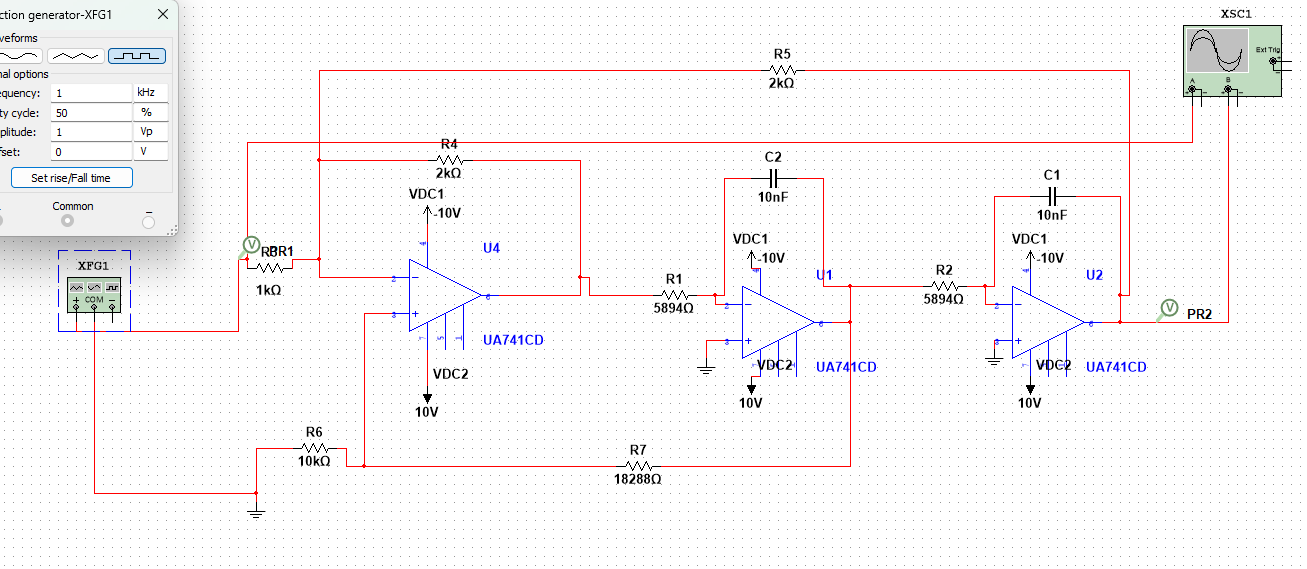
\includegraphics[width=0.8\textwidth]{simulaciones/variables-montaje.png}
    \caption{Montaje Filtro variables de estado}\label{fig:sim-variables-montaje} 
\end{figure}

\begin{figure}[ht]
    \centering
    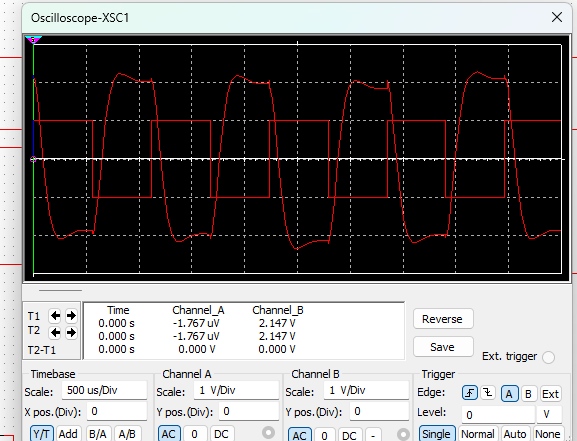
\includegraphics[width=0.8\textwidth]{simulaciones/variables-cuadrada.png}
    \caption{Filtro variables de estado respuesta a onda cuadrada  }
    \label{fig:sim-variables-cuadrada} 
\end{figure}

\begin{figure}[ht]
    \centering
    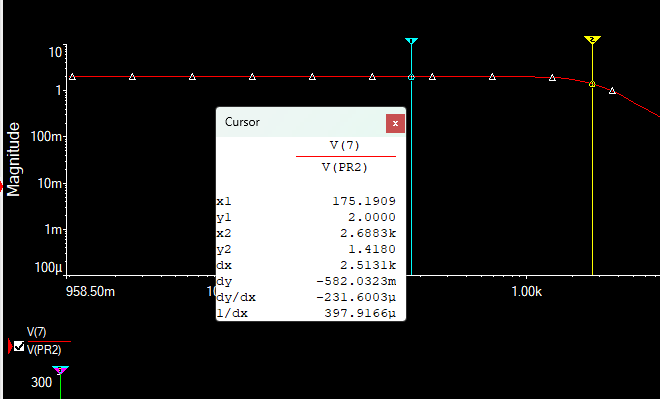
\includegraphics[width=0.8\textwidth]{simulaciones/variables-respuesta.png}
    \caption{Filtro variables de estado respuesta en frecuencia  }
\end{figure}

\FloatBarrier
\subsubsection{Filtro pasa bajos con topología de Sallen-Key}

Para diseñar este filtro partimos de la ecuación \ref{eq:transferencia-pasa-bajo-sallen-key} de la función de transferencia de un filtro pasa bajos con topología de Sallen-Key.

Para la ganancia del filtro, tenemos:

\begin{equation*}
    \gananciaFiltro = K = 2
\end{equation*}

Tenemos:

\begin{equation}
    K = 1 + \frac{R_B}{R_A}
\end{equation}

por tanto:

\begin{align*}
    2 = 1 + \frac{R_B}{R_A}
    1 = \frac{R_B}{R_A}
\end{align*}

\begin{equation*}
    \boxed{R_B = R_A}
\end{equation*}

a estas resistencias les pondremos el valor:

\begin{equation*}
    \boxed{R_B = R_A = 10k\Omega}
\end{equation*}

Ahora seleccionamos los condensadores, por simplicidad podemos hacer

\begin{equation*}
    \boxed{C_2 = C_5 = 10nF}
\end{equation*}

de la función de transferencia obtenemos:

\begin{equation}
    2\factorAmortiguamiento \freqCorte = \left(\frac{1}{R_1 C_2} + \frac{1}{R_4 C_2} + \left(1 - K\right) \frac{1}{R_4 C_5}\right)
\end{equation}

Teniendo en cuenta $C_2 = C_5$ y $K=2$ tenemos:

\begin{equation}
    2\factorAmortiguamiento \freqCorte = \frac{1}{R_1 C_2}
\end{equation}

\begin{align*}
    R_1 &= \frac{1}{2\factorAmortiguamiento \freqCorte C_2} \\
    R_1 &= \frac{1}{2 (0.707) \cdot 2\pi 2.7\times 10^3 \cdot 10\times 10 ^{-9}}
\end{align*}

\begin{equation*}
    R_1 = 4168.76 \Omega
\end{equation*}

Ahora para encontrar $R_2$ tenemos que:

\begin{equation}
    \freqCorte^2 = \frac{1}{R_1 C_1 R_2 C_2} = \frac{1}{R_1 R_2 C_1^2}
\end{equation}

despejando $R_2$ tenemos:

\begin{align*}
    R_2 &= \frac{1}{\freqCorte^2 C_1^2 R_1} \\
    R_2 &= \frac{1}{(2\pi 2.7\times 10^3 \cdot 10\times 10^{-9})^2 \cdot 4168} \\
\end{align*}

\begin{equation*}
    \boxed{R_2 = 8335 \Omega}
\end{equation*}

\begin{figure}[ht]
    \centering
    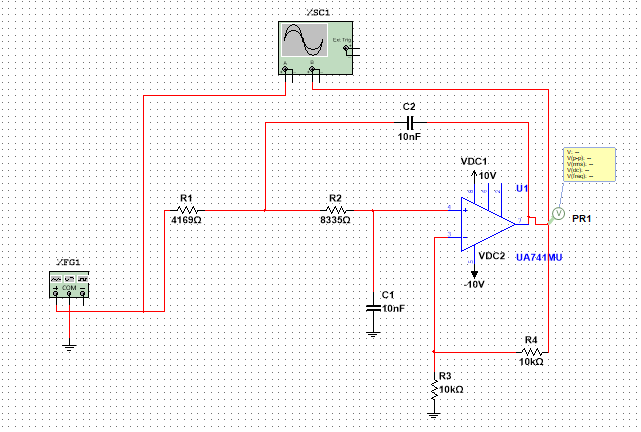
\includegraphics[width=0.8\textwidth]{simulaciones/sallen-montaje.png}
    \caption{Montaje Filtro sallen key}\label{fig:sim-sallen-montaje} 
\end{figure}

\begin{figure}[ht]
    \centering
    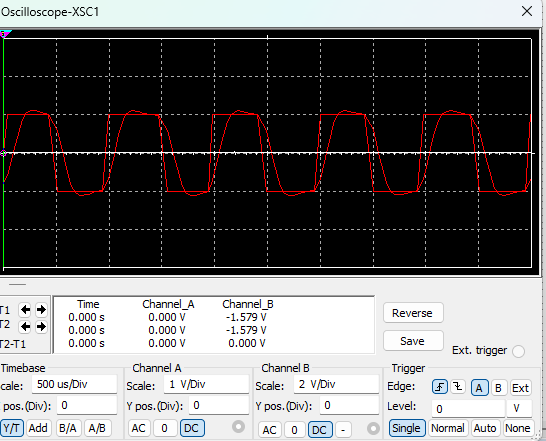
\includegraphics[width=0.8\textwidth]{simulaciones/sallen-cuadrada.png}
    \caption{Filtro sallen key respuesta a onda cuadrada  }
    \label{fig:sim-sallen-cuadrada} 
\end{figure}

\begin{figure}[ht]
    \centering
    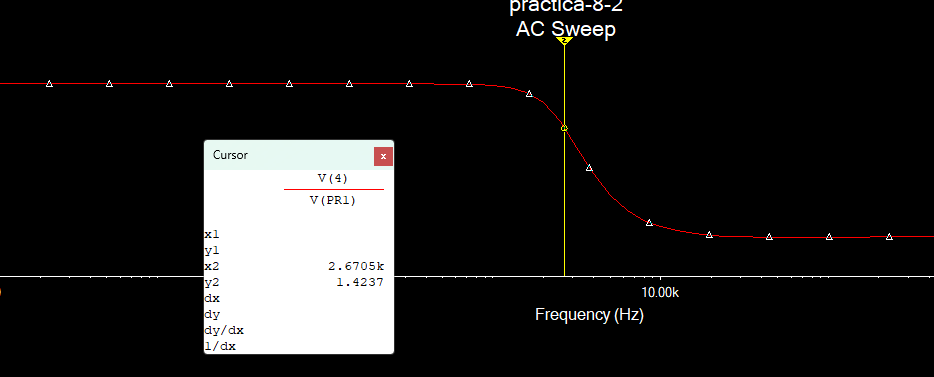
\includegraphics[width=0.8\textwidth]{simulaciones/sallen-respuesta.png}
    \caption{Filtro Sallen key respuesta en frecuencia  }
\end{figure}

\FloatBarrier
\subsubsection{Filtro pasa bajos con realimentación múltiple}

Partiendo de la ecuación \ref{eq:func-transferencia-pasa-bajos-multirealimentacion} de la función de transferencia de un filtro pasa bajos con realimentación múltiple podemos obtener:

\begin{align*}
    H_0 &= \frac{-R_4}{R_1} \\
    R_4 &= - H_0 R_1 \\
\end{align*}

\begin{equation}
    R_4 = 2 R_1\\
    \label{eq:r4-multirealimentacion-pasa-bajos}
\end{equation}

también tenemos que: 

\begin{equation}
    \omega_0 = \sqrt{\frac{1}{R_3 R_4 C_2 C_5}}
    \label{eq:omega-0-multirealimentacion-pasa-bajos}
\end{equation}

Si decimos que: 

\begin{equation*}
    \boxed{C_5 = C_2 = 10nF}
\end{equation*}

la ecuación \ref{eq:omega-0-multirealimentacion-pasa-bajos} se simplifica a:

\begin{equation}
    \omega_0 = \frac{1}{C_2\sqrt{R_3 R_4}}
    \label{eq:omega-0-multirealimentacion-pasa-bajos-simple}
\end{equation}

Por último, tenemos la ecuación:

\begin{equation}
    2\factorAmortiguamiento = \sqrt{\frac{C_5}{C_2}} \left( \sqrt{\frac{R_3}{R_4}} + \sqrt{\frac{R_4}{R_3}} + \frac{\sqrt{R_3 R_4}}{R_1} \right)
    \label{eq:factor-amortiguamiento-multirealimentacion-pasa-bajos}
\end{equation}


que al decir $C_5 = C_2$ entonces la ecuación \ref{eq:factor-amortiguamiento-multirealimentacion-pasa-bajos} se simplifica a:

\begin{equation}
    2\factorAmortiguamiento = \sqrt{\frac{R_3}{R_4}} + \sqrt{\frac{R_4}{R_3}} + \frac{\sqrt{R_3 R_4}}{R_1} 
    \label{eq:factor-amortiguamiento-multirealimentacion-pasa-bajos-simple}
\end{equation}

Ahora, usando la ecuación \ref{eq:omega-0-multirealimentacion-pasa-bajos-simple} en la ecuación \ref{eq:factor-amortiguamiento-multirealimentacion-pasa-bajos-simple} obtenemos:

\begin{equation}
    2\factorAmortiguamiento = \frac{1}{\freqCorte C_2 R_4} + \frac{\freqCorte C_2 R_4}{1} + \frac{1}{\freqCorte R_1 C_2} 
    \label{eq:factor-amortiguamiento-multirealimentacion-pasa-bajos-final}
\end{equation}

Usando \ref{eq:r4-multirealimentacion-pasa-bajos} en la ecuación \ref{eq:factor-amortiguamiento-multirealimentacion-pasa-bajos-final} obtenemos:

\begin{equation}
    2\factorAmortiguamiento = \frac{1}{\freqCorte C_2 2R_1} + \frac{\freqCorte C_2 2R_1}{1} + \frac{1}{\freqCorte R_1 C_2} 
    \label{eq:factor-amortiguamiento-multirealimentacion-pasa-bajos-final-final}
\end{equation}

Todo esto da como resultado:

\begin{align*}
    R_1 &= 1.27k \\
    R_3 &= 640 \\
    R_4 &= 1.88k \\
    C_2 &= 10nF \\
    C_5 &= 100nF \\
\end{align*}

\begin{figure}[ht]
    \centering
    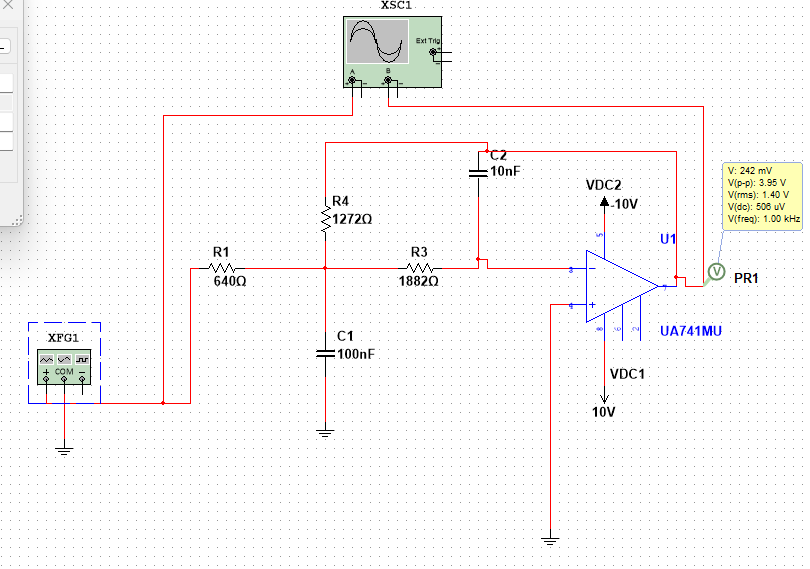
\includegraphics[width=0.8\textwidth]{simulaciones/multirealimentacion-montaje.png}
    \caption{Montaje Filtro multiple realimentación}\label{fig:sim-multirealimentacion-montaje} 
\end{figure}
\begin{figure}[ht]
    \centering
    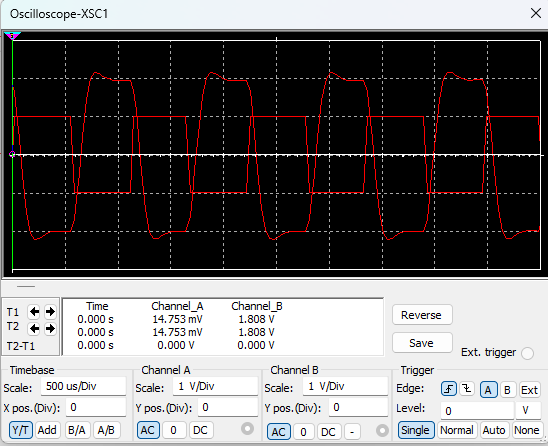
\includegraphics[width=0.8\textwidth]{simulaciones/multirealimentacion-cuadrada.png}
    \caption{Filtro multiple realimentación respuesta a onda cuadrada}
    \label{fig:sim-multirealimentacion-cuadrada} 
\end{figure}
\begin{figure}[ht]
    \centering
    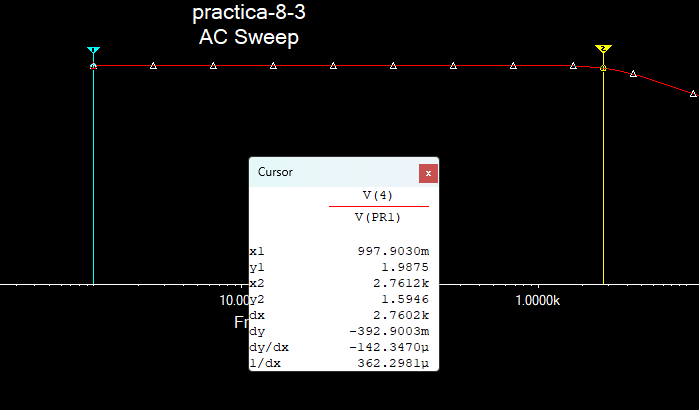
\includegraphics[width=0.8\textwidth]{simulaciones/multirealimentacion-respuesta.png}
    \caption{Filtro multiple realimentación respuesta en frecuencia  }
    \label{fig:sim-multirealimentacion-respuesta} 
\end{figure}